\section{Natural Language Processing (NLP)}
Automatisches erfassen von menschlicher Sprache (gesprochen oder geschrieben). Wichtiger Teilbereich in AI. Ziel ist zu verstehen was ein Mensch will. Kürzlich grössere Fortschritte gemacht. Derzeit ist aber verstehen und auch das Antworten immernoch sehr schwierig für eine KI.\\
Was schon gut funktioniert sind Suchmaschinen, Sprachassistenten(Google Assistant, Alexa) oder Übersetzer (Deepl).
\\
\textcolor{myblue}{Grundlagen Machine-Learning-Projekt:} Die ersten 4 Punkte (Data, Cost-Function, Model, Optimization Procedure) sind die Grundlagen. Die anderen drei benötigt man für verbessertes Machine Learning.
\subsection{Data}
Datenset das gegeben ist inklusive der Pre-Prozess-Pipeline unter anderem mit folgenden Funktionen
\begin{itemize}
\item \textbf{Cleansing}: Aufräumen, Korrigieren und sortieren
\item \textbf{Feature-Engineering}: Extrahieren von Features, z.B Katze ist ein Säugetier (Beziehungen)
\item \textbf{Data-Argumentation}: Daten vervielfältigen durch manipulation (Spiegeln, Farbänderung) oder hinzufügen neuer Date
\end{itemize}

\subsection{Cost-Function (Loss)}
Mathematischer Ausdruck der sagt wie gut oder schlecht Aufgabe gelöst wurde. Dies anhand Angabe einer Zahl. Mean Squared Error (MSE) wird häufig genutzt. Weiter gibt es Domain-Spezifische Kosten.
\\
Beispiel: Gesichtserkennungsalgorithmus. Nun muss man Kosten schätzen wenn Gesichtserkennung falsch positiv oder falsch
negativ ist. Je nach Ort kann es andere Auswirkungen haben. (Access-Control bei CIA oder Identifizierung von Kunden, die viel
Geld ausgeben in einem Geschäft)
\subsection{Model}
Der Teil, der aus einem Input einen Output generiert. Kann einfach sein (Linear yi = axi + b) oder komplexes neuronalesNetzwerk mit Millionen von Parameter.
\\
Typischerweise verwendet man Framework wie Tensorflow oder Pytorch
\\
Unterschiedliche Aufgaben benötigen unterschiedliches Modell (Regression, Entscheidungsbaum)
\subsection{Optimization Procedure}
Modell muss nun durch Machine-Learning optimiert werden. Dazu braucht es einen Algorithmus. Optimierungsprozedur nimmt alle oben genannte Elemente und schraubt so lange an Parameter rum, bis das optimale Ergebnis rauskommt.
\\
Beispiele: Stochastic Gradient Descent (SGD), ADAM, RMSProp, ...
\subsection{Performance Optimization}
Bauen von effizienten Pipelines ist schwierig. Deshalb sollten Tool-spezifische Empfehlungen und Referenz-Implementationen zur Hilfe genommen werden.
\subsection{Visualization and evaluation of the Learning Process}
Man kann Lernprozess visualisieren. Man kann also Zeigen ob der Optimierer was sinnvolles tut. Hier kann Tensorboard genutzt werden.
\subsection{Cross-Validation und Regularization}
Ziel ist Modelle zu trainieren, die Gut generalisieren. AI soll eine gewisse Flexibilität haben. \\
Beispiel: Hundebilderkenner soll auch neue Hunderaussen automatisch erkennen.
\subsection{}
Am einfachsten nutzt man dazu Vektoren, welche Wörter auf Grund Ihrer Meinung intepretieren.
\subsection{Vorgehen 1: One-Hot Representation}
Jedem Wort wird ein Vektor zugewiesen mit einem einzigen 1 Wert und alle anderen Werte auf 0 gesetzt.\\
Vektordimeinsion = Anzahl unterschiedliche Wörter
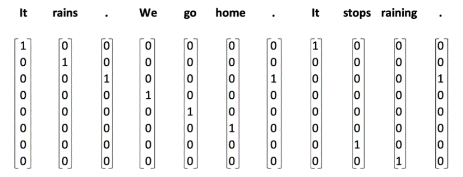
\includegraphics[width=\linewidth]{img/one-hot.png}
Nachteile:
\begin{itemize}
\item \textbf{High dimensional}: Vektoren können schnell sehr grosswerden (Wikipedia-Artikel hat schnell 100'000 Wörter)
\item \textbf{Sparse}: Jeder Vektor hat nur eine 1 und dann viele Nullen. (1 zu 99'999 im Wikipediabeispiel). Sind sehr Memory-Ineffizient und KI kann davon nicht viel lernen
\item \textbf{No generalization}: Es fehlt der Kontext. Alle Wörter sind unabhängig voneinander und es kann keine Bedeutung abgeleitet werden (Z.B Ananas und Birne sind Essen)
\end{itemize}
\subsection{Vorgehen 2: Indexing}
Man macht eine Liste von Wörter und weist diese eine Nummer zu. So benötigt ein Satz nur ein einziger Vektor. Sehr ähnlich wie der One-Hot-Vektor. Aber etwas besser. Deshalb wird Indexing meist als Preprocessing-Step genutzt.
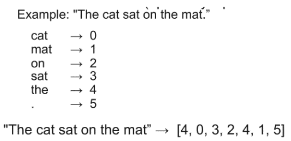
\includegraphics[width=\linewidth]{img/indexing.png}
\subsection{Vorgehen 3: Distributed Representation (dense vectors)}
Ein Wort kann definiert werden mit einem Kontext. Wörter mit ähnlicher Schematik teilen oft den Kontext (cat and rat = Animals)
\\\\
Beispiel: "Look at that little furry mukawibuu with white paws climbing a tree" $\rightarrow$ Mukawibuu wird wohl einem Koala ähneln
\\\\
Bei Distributed Representation wird dieses Konzept genutzt gemacht. Ein Wort, welches indexiert wurde, wird mit einem Algorithmus (Embedding Layer) zu einem Vektor umgewandelt.
\\
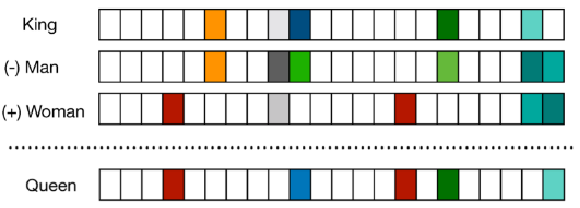
\includegraphics[width=\linewidth]{img/distrubuted-representation.png}
\\
Mit guten Vektoren kann man dann durch Mathematik Ähnlichkeiten erkennen oder durch Addition/Subtraktion neue Wörter bilden. Dazu wird das Skalarprodukt verwendet. Somit kann der Computer mittels Mathematik die Ähnlichkeiten von unterschiedlichen Wörter erkennen.

\begin{itemize}
\item Skalarprodukt zwischen zwei Vektoren ist maximal, wenn beide in die selbe Richtung zeigen
\begin{itemize}
\item Haben beide Vektoren die Norm 1, dann ist das Maximum 1
\end{itemize}
\item Skalarprodukt zwischen zwei Vektoren ist null, wenn die Vektoren senkrecht (orthogonal) zueinander stehen
\item Skalarprodukt zwischen zwei Vektoren ist minimal (negativ), wenn beide Vektoren in entgegengesetzte Richtung zeigen
\begin{itemize}
\item Haben beide Vektoren die Norm 1, dann ist das Minimum -1
\end{itemize}
\end{itemize}

\subsection{Cosine Distance (Kosinusdistanz)}
Das Skalarprodukt wird verwendet für die Cosine-Distance (Kosinusdistanz). Ähnliche Wörter haben eine ähnliche Kosinusdistanz.
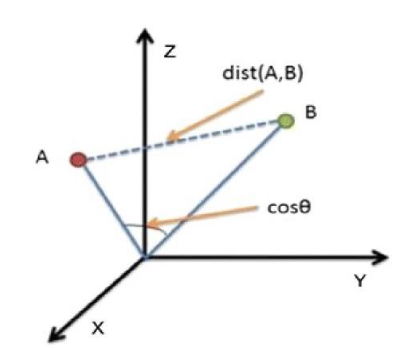
\includegraphics[width=\linewidth]{img/cosine_distance1.png}
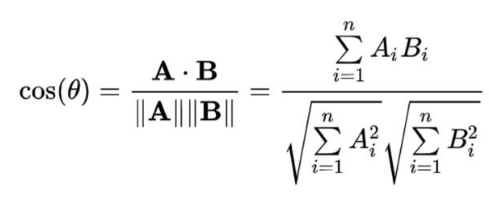
\includegraphics[width=\linewidth]{img/cosine_distance2.png}

\textcolor{myblue}{Skalarprodukt:}\\
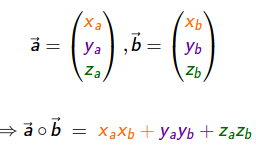
\includegraphics[width=\linewidth]{img/skalarprodukt.png}
$$\frac{dotP\left(e,m\right)}{norm\left(e\right)\cdot norm\left(m\right)}$$
Vektor erstellen = Menu -> 7 -> 1
dotP = Menu -> 7 -> C -> 3\\
norm = Menu -> 7 -> 7 -> 1\\

\subsection{Rechenbeispiel}
Berechne die Kosinusdistanz zwischen Elefant und Maus, sowie zwischen Elefant und Bike.\\
Im Taschenrechner kann folgende Formel gebraucht werden:\\
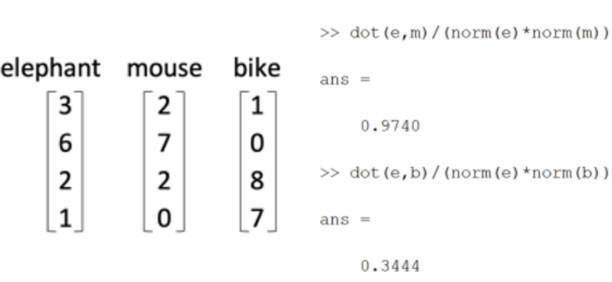
\includegraphics[width=\linewidth]{img/elefant_maus.png}
Elefant und Maus sind sich sehr ähnlich, weshalb die Kosinusdistanz mit 0.974 nahe bei 1 ist. Elefant und Bike ähneln sich nicht.